% ------------------------------------------------------------------------
% CS198 Final Paper
% Project Title: <insert title>
% Authors: < your names >
% Date Submitted: May 17, 2018
%
% ------------------------------------------------------------------------
\documentclass[letterpaper,12pt]{report}
\usepackage[centertags]{amsmath}
\usepackage{amsfonts}
\usepackage{amssymb}
\usepackage{amsthm}
\usepackage{newlfont}
\usepackage{epsfig}

\usepackage{booktabs}
\usepackage{array}
\usepackage[hidelinks]{hyperref}
\hypersetup{
   colorlinks=false,
   urlcolor=black,    % color of external links
   linkcolor=black,  % color of toc, list of figs etc.
   citecolor=black,   % color of links to bibliography
}

\usepackage{UPCS198} %UP Dept. of Computer Science CS198 Style
\usepackage{UPCSINC1}
\usepackage[active]{LTX}

\makeatletter
\def\@xfloat#1[#2]{\ifhmode \@bsphack\@floatpenalty -\@Mii\else
   \@floatpenalty-\@Miii\fi\def\@captype{#1}\ifinner
      \@parmoderr\@floatpenalty\z@
    \else\@next\@currbox\@freelist{\@tempcnta\csname ftype@#1\endcsname
       \multiply\@tempcnta\@xxxii\advance\@tempcnta\sixt@@n
       \@tfor \@tempa :=#2\do
			{\if\@tempa h\advance\@tempcnta \@ne\fi
			 \if\@tempa t\advance\@tempcnta \tw@\fi
			 \if\@tempa b\advance\@tempcnta 4\relax\fi
			 \if\@tempa p\advance\@tempcnta 8\relax\fi
	 }\global\count\@currbox\@tempcnta}\@fltovf\fi
    \global\setbox\@currbox\color@vbox\normalcolor\vbox\bgroup
    \def\baselinestretch{1}\@normalsize
    \boxmaxdepth\z@
    \hsize\columnwidth \@parboxrestore}
\makeatother

\hfuzz2pt
\newlength{\defbaselineskip}
\setlength{\defbaselineskip}{\baselineskip}
\newcommand{\setlinespacing}[1]
           {\setlength{\baselineskip}{#1 \defbaselineskip}}
\newcommand{\doublespacing}{\setlength{\baselineskip}
                           {2.0 \defbaselineskip}}
\newcommand{\singlespacing}{\setlength{\baselineskip}{\defbaselineskip}}
% MATH -------------------------------------------------------------------
\newcommand{\A}{{\cal A}}
\newcommand{\h}{{\cal H}}
\newcommand{\s}{{\cal S}}
\newcommand{\W}{{\cal W}}
\newcommand{\BH}{\mathbf B(\cal H)}
\newcommand{\KH}{\cal  K(\cal H)}
\newcommand{\Real}{\mathbb R}
\newcommand{\Complex}{\mathbb C}
\newcommand{\Field}{\mathbb F}
\newcommand{\RPlus}{[0,\infty)}
\newcommand{\norm}[1]{\left\Vert#1\right\Vert}
\newcommand{\essnorm}[1]{\norm{#1}_{\text{\rm\normalshape ess}}}
\newcommand{\abs}[1]{\left\vert#1\right\vert}
\newcommand{\set}[1]{\left\{#1\right\}}
\newcommand{\seq}[1]{\left<#1\right>}
\newcommand{\eps}{\varepsilon}
\newcommand{\To}{\longrightarrow}
\newcommand{\RE}{\operatorname{Re}}
\newcommand{\IM}{\operatorname{Im}}
\newcommand{\Poly}{{\cal{P}}(E)}
\newcommand{\EssD}{{\cal{D}}}
% THEOREMS ---------------------------------------------------------------
\theoremstyle{plain}
\newtheorem{thm}{Theorem}[section]
\newtheorem{cor}[thm]{Corollary}
\newtheorem{lem}[thm]{Lemma}
\newtheorem{prop}[thm]{Proposition}
\theoremstyle{definition}
\newtheorem{defn}{Definition}[section]
\theoremstyle{remark}
\newtheorem{rem}{Remark}[section]
\numberwithin{equation}{section}
\renewcommand{\theequation}{\thesection.\arabic{equation}}
\setlength{\tclineskip}{1.05\baselineskip}


\begin{document}

%\nobib
%\draft
%\nofront

\permissionfalse


\submityear{May 2026}

% ------------------------------------------------------------------------
\title{ATHENA: An Image Captioning Pipeline for Constrained Underwater Environments}


\cs198 
\author{Rodrigo Emmanuel D. Roy \\
        Krisha Anne E. Chan
}

\newcommand\authorline{Rodrigo Emmanuel D. Roy and Krisha Anne E. Chan}

\degreeinitial{BS Computer Science} % put here your previous degree
\major{Computer Science}
\adviser{Prof. Prospero C. Naval, Jr., Ph.D.}
% \adviser{Asst. Prof. Carlo R. Raquel}
% \adviser{Asst. Prof. Roselyn S. Gabud}
% \adviser{Asst. Prof. Paul Rossener R. Regonia, D.Sc.}
\secondreader{Asst. Prof. Carlo R. Raquel} % uncomment for two advisers
% \dean{Dean Maria Antonia N. Tanchuling, Ph.D.}

% ------------------------------------------------------------------------
{
\forgeterr{?0000} % Don't bother with over/under-full boxes
\beforepreface
\forgeterr{?1111} % Process All Errors from Here on
}
% ------------------------------------------------------------------------
{
\typeout{Abstract}
\prefacesection{Abstract}

Autonomous underwater vehicles (AUVs) are constrained by low-bandwidth communication channels, as well as limited onboard computation. Current approaches either rely heavily on cloud processing or transmitting raw images, which are infeasible on untethered AUVs. In this work, we introduce ATHENA: AI Transformer for Hydro-Environmental Navigation and Analysis, an edge-capable Vision-Language Model (VLM) pipeline that can enable AUVs to describe underwater scenes as text, allowing for efficient data transmission and real-time situational awareness. To address common underwater challenges such as color distortion, light attenuation, and haze, we apply a multi-step preprocessing pipeline that enhances image clarity for the VLM. By leveraging 4-bit quantization, ATHENA reduces the memory footprint to just 652.86 MB, making it deployable on embedded hardware. Preliminary results show concise, accurate captions with significant improvements on standard image captioning benchmarks such as BLEU, ROUGE-L, and CIDEr.

% Tips on how to write abstract:
% https://communities.springernature.com/posts/how-to-write-an-abstract
% https://unl.libguides.com/c.php?g=51569&p=2633458
}
% ------------------------------------------------------------------------
{
\typeout{Acknowledgements}
\prefacesection{Acknowledgement}

It is customary to thank your research collaborators, adviser(s), friends, etc.
Mentioning your pet cat, dog, lizard, etc. is optional.
}
% ------------------------------------------------------------------------
\afterpreface
\def\baselinestretch{1}
\setlinespacing{1.66}
% ------------------------------------------------------------------------
{
%\typeout{Introduction}
%\include{introd}
}
% ------------------------------------------------------------------------
\setlinespacing{1.66}
% ------------------------------------------------------------------------

\chapter{Introduction} \label{sec:intro}
Autonomous underwater vehicles (AUVs) are increasingly deployed for marine exploration, environmental monitoring, and subsea infrastructure inspection. Long-duration autonomous missions require onboard perception systems that can summarize visual scenes and transmit only essential information to remote operators. However, this is constrained by two defining characteristics of underwater robotics: severely limited communication bandwidth and restricted onboard computational resources~\cite{lowbandwith}. Underwater communication is typically achieved via acoustic channels, which use sound waves to transmit information over long distances, since radio signals attenuate rapidly in water and optical signals require line-of-sight. Acoustic channels have low bandwidth, high latency, and multipath interference, making raw or high-resolution image transmission and cloud-based processing impractical, especially for untethered AUVs~\cite{chen1}\cite{li2}\cite{zhang3}. Many state-of-the-art vision models also exceed the compute and memory budgets of embedded AUV hardware~\cite{li2}\cite{marafioti4}.

Underwater imagery further complicates perception due to light attenuation, scattering, haze, and color distortion, which vary with depth, turbidity, and lighting conditions. Prior work highlights the need for enhancement and restoration pipelines to address these challenges before downstream processing~\cite{li2}.

To overcome these limitations, recent approaches focus on conveying semantic content rather than raw images. Textual descriptions offer a compact, bandwidth-efficient alternative~\cite{chen1}\cite{zhang3}. Vision-language models (VLMs) such as those deployed in SINGER~\cite{singer} and SmolVLM~\cite{marafioti4} demonstrate the feasibility of onboard semantic understanding, though existing architectures are often too large for edge deployment or are not tailored to underwater imagery.

Inspired by these works, we propose ATHENA, an edge-capable underwater scene captioning system that enhances raw images and produces concise textual descriptions suitable for low-bandwidth transmission, enabling AUVs to communicate semantically meaningful information in real time.

The remainder of this paper is organized as follows: Chapter~2 reviews related work on vision-language models, semantic communication, and underwater image enhancement. Chapter~3 presents the ATHENA framework, including the dataset, methodology, and experimental setup. Chapter~4 details experiments and analyzes results. Finally, Chapter~5 concludes the paper.

\section{Statement of the Problem}

Existing underwater image captioning approaches face three interconnected challenges. First, most state-of-the-art VLMs are pre-trained on terrestrial image datasets and consistently underperform on underwater scenes due to the significant domain gap caused by color attenuation, backscatter, and turbidity~\cite{mainref}. Second, underwater imagery is inherently degraded by haze, low contrast, and scattering, and current enhancement methods lack consistency across diverse underwater conditions~\cite{7steppipeline}. Third, AUVs operate under strict onboard computational and memory budgets and rely on low-bandwidth acoustic communication channels, making cloud-based processing and raw image transmission infeasible for real-time operation~\cite{lowbandwith}.

\section{Significance of this Study}

This study addresses the need for a practical, edge-deployable system that enables AUVs to communicate the semantic content of underwater scenes without relying on high-bandwidth channels or cloud processing. By introducing ATHENA, an edge-capable VLM pipeline with domain-adaptive fine-tuning and a tailored image enhancement pipeline, this work advances the state of the art in underwater image captioning and demonstrates that compact, quantized VLMs can achieve competitive performance on standard benchmarks while meeting the resource constraints of embedded AUV hardware. The findings contribute to the broader effort of enabling long-duration autonomous underwater missions with onboard, real-time scene understanding.

\section{Scope of this Study}

This study focuses on image captioning for underwater scenes using two datasets: the Li et al.\ dataset of 3,176 underwater images with five human-annotated captions each~\cite{mainref}, and UWBench~\cite{uwbench}, a large-scale benchmark of 15,003 high-resolution images with expert-verified captions covering 158 object categories. Three VLM backbones are evaluated: SmolVLM-Instruct, BLIP-2 OPT 2.7B, and Qwen3.5-VL, under a systematic ablation across LoRA ranks and DoRA configurations. The image enhancement pipeline is based on a seven-step protocol adapted from Wang et al.~\cite{7steppipeline}, with CLAHE substituted for the original contrast stretching step. Deployment feasibility is assessed under 4-bit NF4 quantization targeting embedded edge hardware. This work does not address real-time physical deployment on AUV hardware, underwater object detection, video captioning, or the design of acoustic communication protocols.


\chapter{Review of Related Literature} \label{sec:rrl}
Recent advances in autonomous robotics and computer vision have explored various approaches for perception, communication, and image enhancement. In the context of underwater scene understanding, three main areas are particularly relevant: vision-language models (VLMs) for robotic perception, semantic communication methods for low-bandwidth environments, and specialized techniques for underwater image enhancement.

\section[Paull, Huang, Seto \& Leonard]{Communication-Constrained Multi-AUV Cooperative SLAM~\cite{lowbandwith}}
Multi-AUV cooperative SLAM enables collaborative localization through direct encounters (relative range measurements) and indirect encounters (shared observations of seabed features). However, underwater acoustic channels operate at approximately 1,500 m/s propagation speed with throughputs of only 10--100 bytes per second, 20--50\% packet dropout, and TDMA constraints, making raw sensor data transmission impractical. A graph-based C-SLAM algorithm addresses this by locally marginalizing vehicle pose estimates via the Schur complement, condensing accumulated observations into compact virtual measurements. A sparsification step based on constrained convex optimization further reduces packet size by minimizing the Kullback-Leibler divergence between the original and approximate distributions while enforcing a predetermined sparse Jacobian structure. The resulting payload scales linearly with observed features and remains constant in time even under dropped packets. Simulation with two AUVs demonstrates bounded localization error at 50\% dropout with a maximum packet size of 192 bytes per 10-second interval.

These severe bandwidth constraints directly motivate ATHENA's semantic captioning approach: if even compressed SLAM packets must remain under 200 bytes to be acoustically viable, transmitting compact natural language scene descriptions is far more practical than any form of image transmission.

\section[Luo, Zhou, Zeng, Jiang, Qi, Xiang, Pang \& Tang]{Robotics Perception and Control: Key Technologies and Applications~\cite{perception}}
This comprehensive review surveys nine sensor categories used in robotic control systems, including IMUs, visual sensors, LiDAR, tactile sensors, and EMG sensors, categorized as either proprioceptive (measuring internal robot states) or exteroceptive (gathering information from the external environment). Vision sensors occupy a central role, supporting object recognition, visual SLAM, autonomous navigation, medical surgery, and deep learning-based robotic grasping across industrial, medical, and exploratory domains.

The survey situates VLMs as an emerging class of exteroceptive perception module that converts visual input into structured semantic representations for downstream tasks such as navigation and scene understanding. ATHENA adopts this paradigm by deploying a VLM as an onboard sensor module that produces textual descriptions suitable for transmission over low-bandwidth acoustic channels, analogous to how onboard ATR systems convert raw sonar returns into compact feature representations.

\section[Li \& Zhang]{Real-Time Vision--Language Analysis for Autonomous Underwater Drones~\cite{li2}}
A cloud-edge framework for real-time VLM analysis in AUVs uses Qwen2.5-VL, a 72-billion-parameter model, by offloading inference to a cloud server while retaining lightweight preprocessing on the edge device. The edge performs frame sampling at 1 fps and a three-stage image enhancement pipeline (color correction, backscatter reduction, white balance), while communication relies on a 5 Mbps fiber-optic link with adaptive JPEG quality scaling and bounded frame buffering. Simulation across pipeline inspection, coral reef monitoring, and wreck investigation scenarios demonstrates consistent scene comprehension with end-to-end latencies near 1 second.

However, the reliance on cloud infrastructure and tethered optical fiber makes this approach unsuitable for untethered AUV operations, underscoring the need for a fully onboard, lightweight inference pipeline such as the one adopted in ATHENA.

\section[Adang, Low, Shorinwa \& Schwager]{SINGER: An Onboard Generalist Vision-Language Navigation Policy for Drones~\cite{singer}}
SINGER addresses open-vocabulary drone navigation by integrating a photorealistic language-embedded 3D Gaussian Splatting simulator, an RRT*-based trajectory generator, and a lightweight visuomotor policy trained on synthetic data. The system uses CLIPSeg to convert RGB images into semantic heatmaps as policy inputs, enabling generalization across unseen environments. To achieve real-time inference on the NVIDIA Jetson Orin Nano 8GB, CLIPSeg is traced to ONNX and executed via the CUDA runtime at 12 Hz. Hardware experiments demonstrate 76.67\% goal proximity success across 30 trials, outperforming a classical PD controller baseline by 23.33\% with 10\% fewer collisions.

This result establishes a key precedent for ATHENA's edge deployment strategy, confirming that VLM-based semantic understanding can run in real time on the Jetson Orin Nano without cloud offloading and validating the hardware feasibility of onboard inference in resource-constrained robotic platforms.

\section[Marafioti et al.]{SmolVLM: Redefining Small and Efficient Multimodal Models~\cite{marafioti4}}
SmolVLM is a family of compact multimodal models that systematically investigates architectural configurations, tokenization strategies, and data composition to maximize VLM performance at minimal memory footprints. The architecture pairs a SigLIP vision encoder with a SmolLM2 language backbone and uses pixel shuffle compression to reduce visual tokens by a factor of 16. Three variants are produced: SmolVLM-256M ($<$ 1 GB RAM), SmolVLM-500M (1.2 GB), and SmolVLM-2.2B (4.9 GB). The 2.2B model achieves 59.8\% average score across nine benchmarks using only 4.9 GB VRAM, outperforming Qwen2VL-2B which requires 13.7 GB. SmolVLM-256M, operating under 1 GB RAM, significantly surpasses the 80B Idefics model despite a 300-fold parameter gap.

SmolVLM-Instruct serves as the lightweight backbone evaluated in ATHENA, representing the sub-1 GB end of the model scale spectrum and confirming that competitive captioning performance is achievable within the memory budgets of embedded AUV hardware.

\section[J. Li, D. Li, Savarese \& Hoi]{BLIP-2: Bootstrapping Language-Image Pre-Training with Frozen Image Encoders and Large Language Models~\cite{blip2}}
BLIP-2 proposes a compute-efficient pre-training strategy that bootstraps vision-language learning from frozen image encoders and frozen LLMs using a lightweight Querying Transformer (Q-Former) with only 188 million trainable parameters, 54 times fewer than Flamingo80B, while surpassing it by 8.7\% on zero-shot VQAv2. Q-Former employs 32 learned query vectors to extract task-relevant visual information through cross-attention, serving as an information bottleneck between the vision and language components. The model is pre-trained in two stages: first learning visual representations through contrastive, generative, and matching objectives on a 129M-image dataset; then projecting Q-Former outputs as soft visual prompts to a frozen LLM for language generation. On zero-shot captioning, BLIP-2 achieves a CIDEr score of 121.6 on the NoCaps validation set.

However, systematic analyses identify BLIP-2 as producing formulaic outputs with low lexical diversity and limited reasoning consistency~\cite{hani2026systematic}. In ATHENA, BLIP-2 OPT 2.7B serves as the intermediate-scale backbone in the ablation study, providing a reference point between SmolVLM and Qwen3.5-VL.

\section[Hani, Tagougui \& Kherallah]{Toward Human-Level Understanding: A Systematic Review of Vision-Language Models for Image Captioning~\cite{hani2026systematic}}
A systematic review evaluates eight VLMs for image captioning under zero-shot conditions on MS-COCO, combining automatic metrics (CLIPScore, perplexity, lexical diversity) with human evaluation across 1,000 captions per model. LLaVA achieves the highest CLIPScore (0.757), while BLIP-2 exhibits the lowest lexical diversity and highest perplexity (97.1), characteristic of its conservative Q-Former bottleneck. A structured WH-question analysis across six semantic dimensions (Subject Detail, Action Detail, Location Detail, Time Detail, Manner Detail, and Purpose/Reasoning) reveals a clear progression from early models producing basic subject-action-location statements to advanced models generating multi-component narratives approaching human-level descriptive richness.

Critically, the review identifies that VLMs pre-trained on terrestrial datasets consistently struggle with domain-shifted inputs, exhibiting degraded performance on imagery with fundamentally different visual statistics. This finding directly motivates ATHENA's fine-tuning strategy: standard zero-shot VLMs cannot produce accurate underwater scene descriptions without supervised adaptation on domain-specific data.

\section[NVIDIA]{TensorRT-LLM: Embedded Inference for Large Vision-Language Models~\cite{tensorrt}}
The TensorRT Edge-LLM framework provides tooling for deploying large language and vision-language models on embedded hardware through aggressive quantization and inference optimization. Targeting devices such as the NVIDIA Jetson family, the framework applies INT4 and INT8 weight quantization, KV-cache compression, and attention kernel fusion to reduce memory footprint and inference latency. Its 4-bit weight quantization achieves approximately 4$\times$ memory reduction compared to FP16 inference, making large VLMs viable on platforms with limited unified memory.

Support for Qwen3.5-VL through this framework justifies its selection as a viable ATHENA backbone despite its larger parameter count, with 4-bit NF4 quantization via the \textit{bitsandbytes} library confirming deployment feasibility on the Jetson Orin hardware platform.

\section[H. Li, Wang, Zhang, L. Li \& Ren]{Underwater Image Captioning: Challenges, Models, and Datasets~\cite{mainref}}
Underwater image captioning is hindered by three challenges: models pre-trained on terrestrial images create a systematic domain gap that causes misidentification of marine objects; underwater images exhibit degraded quality from wavelength-dependent absorption, backscatter, and turbidity; and existing underwater datasets either lack captions or are too small for training. The proposed UICM-SOFF model addresses these by using a physics-based submergence GAN to generate 80,000 degraded training images, pre-training a Meta-ResNeXtor feature extractor via meta-learning, and fusing scene-level features with YOLOv8 object-level features through a cross-attention Transformer encoder. The constructed dataset comprises 3,176 images across ten categories (predominantly fish, coral reefs, and divers) with five human-written captions each, totaling 15,880 captions.

This dataset serves as the primary training and evaluation benchmark for ATHENA, and UICM-SOFF's scores (BLEU-1: 0.7249, BLEU-4: 0.3953, ROUGE-L: 0.5888, CIDEr: 1.2831) define the state-of-the-art baseline against which ATHENA's results are directly compared.

\section[W. Chen, Xu, H. Chen, X. Zhang, Qin, Y. Zhang \& Han]{Semantic Communication Based on Large Language Model for Underwater Image Transmission~\cite{chen1}}
An LLM-based semantic communication framework for underwater image transmission represents image content as compact semantic information rather than pixel data, reducing transmitted data to approximately 0.8\% of the original image size. The semantic encoder passes the image to a visual LLM to generate text encoding high-level content, identifies key image regions via bounding box prediction at reduced resolution, and aggressively resamples the remaining background; the combined payload is approximately 27,525 bytes versus the original 3,145,728 bytes. At the receiver, a diffusion model reconstructs the full image from three guidance signals conditioned on the recovered text and key regions. Evaluation on the SUIM dataset shows the highest CLIP scores across all tested SNR levels (0--18 dB).

Both this framework and ATHENA share the core insight that language-based representations serve as an effective acoustic communication payload to overcome the fundamental bandwidth limitations of underwater channels.

\section[Zhang et al.]{An Underwater Acoustic Semantic Communication Approach to Underwater Image Transmission~\cite{zhang3}}
This work proposes an acoustic semantic communication framework that extracts semantic features from underwater images using deep neural networks and encodes them for delivery over bandwidth-limited, high-latency acoustic channels. Semantic encoding separates task-relevant content from perceptually redundant detail, achieving significant bandwidth savings while maintaining downstream task performance under challenging acoustic conditions.

These findings reinforce the practical viability of semantic representations for AUV communication and provide quantitative support for ATHENA's design choice to transmit VLM-generated captions rather than compressed images over acoustic channels.

\section[Luo, Chen \& Guo]{Semantic Communications: Overview, Open Issues, and Future Research Directions~\cite{luo2022semantic}}
A broad survey of semantic communication systems identifies three communication levels: technical (reliable bit transmission), semantic (accurate meaning transfer), and effectiveness (achieving desired receiver effects). Semantic systems encode only semantically relevant content while discarding redundant data, which is particularly valuable in bandwidth-constrained environments such as underwater acoustic channels where available bitrates are orders of magnitude lower than those needed for raw image transmission.

This framework underpins the rationale for ATHENA's use of VLM-generated captions as the communication payload: by transmitting meaning rather than pixel representations, ATHENA operates as a semantic communication system at the second level, achieving efficiency gains through language-level scene representation.

\section[Shi, Xiao, Li \& Xie]{From Semantic Communication to Semantic-Aware Networking: Model, Architecture, and Open Problems~\cite{shi2021semantic}}
Semantic-aware networking decouples semantic encoding from physical-layer transmission, enabling network resources to be allocated based on semantic importance rather than treating all bits uniformly. The proposed architecture introduces a semantic source encoder, a channel encoder, and a semantic decoder that reconstructs intended meaning without necessarily recovering original data exactly. Unlike conventional compression, which minimizes bitrate subject to distortion constraints, semantic encoding minimizes the information needed to achieve a specified level of semantic fidelity.

This decoupled architecture supports ATHENA's goal of generating compact captions that can be prioritized for transmission over low-bandwidth acoustic channels, where operator situational awareness depends on scene content rather than image fidelity.

\section[Xie, Qin, Li \& Juang]{Deep Learning Enabled Semantic Communication Systems~\cite{xie2021deep}}
End-to-end deep learning methods can jointly optimize semantic encoding and channel coding, outperforming conventional bit-based communication under low SNR conditions. The system trains a semantic encoder-decoder pair with the channel as a non-trainable intermediate, learning which input aspects are most important for downstream tasks and encoding them more robustly. Experiments show significant improvements in semantic fidelity at low SNR values typical of underwater acoustic channels.

This lends support to ATHENA's use of text captions as a robust underwater transmission format, since natural language descriptions constitute a compact semantic representation that preserves task-relevant content more reliably than compressed image data under noisy channel conditions.

\section[Huang, Tao, Gao \& Lu]{Deep Learning-Based Image Semantic Coding for Semantic Communications~\cite{huang2021deep}}
A deep learning-based framework transmits semantic image representations rather than compressed pixel data through joint source-channel coding. The semantic encoder learns scene-level abstractions appropriate for downstream tasks while discarding irrelevant texture detail, and the decoder uses generative modeling to reconstruct images from the compact semantic code. The approach scales to very low bitrate regimes corresponding to the available bandwidth of underwater acoustic channels.

While this framework transmits learned continuous-valued semantic features, ATHENA extends the same principle to discrete natural language representations: VLM-generated captions encode the semantically relevant aspects of underwater scenes in a format that is both human-interpretable and efficiently transmissible over acoustic channels.

\section[J. Wu, C. Wu, Lin, Yoshinaga, Zhong, Chen \& Ji]{Semantic Segmentation-Based Semantic Communication System for Image Transmission~\cite{wu2023semantic}}
This system applies semantic segmentation as the transmission representation for image communication, extracting pixel-level semantic labels instead of raw pixels. Segmentation maps require significantly lower bitrates while preserving object category distribution and scene structure, sufficient for many monitoring and inspection tasks. The system demonstrates robust performance under channel noise conditions typical of wireless and acoustic links.

This approach contextualizes ATHENA's choice of natural language captions as a compact alternative: while segmentation maps encode spatial structure, captions encode semantic content in a directly human-readable form that can be interpreted without specialized decoding equipment, making them well-suited for transmission to surface operators.

\section[Akkaynak \& Treibitz]{Sea-thru: A Method For Removing Water From Underwater Images~\cite{seathru}}
Underwater images suffer from systematic color distortion and contrast loss caused by wavelength-dependent absorption and scattering. Sea-thru addresses these by proposing a physics-based image formation model that separates signal attenuation from backscatter as functions of range-to-scene depth. By estimating and subtracting the backscatter contribution, then compensating for channel-specific attenuation, the method recovers true object reflectances validated against photographs taken in air.

However, the requirement for depth information, typically obtained from multi-image structure-from-motion reconstruction, limits real-time onboard applicability. The method also does not address contrast or sharpness degradation beyond color correction. These limitations motivate the more comprehensive multi-step enhancement pipeline adopted in ATHENA, which addresses color, contrast, and sharpness without requiring depth information.

\section[Wang, Sun \& Ren]{Meta Underwater Camera: A Smart Protocol for Underwater Image Enhancement~\cite{7steppipeline}}
Underwater images suffer from three categories of degradation: color deviations from wavelength-dependent attenuation, low contrast from light scattering, and detail blur from backscatter. The Meta Underwater Camera (MUC) protocol addresses all three through a cascaded seven-step pipeline: (1) attenuated channel compensation, (2) white balance via YCbCr mean method, (3) tone mapping, (4) HSL saturation adjustment, (5) contrast stretching, (6) gamma correction, and (7) high-pass fusion. A reinforcement learning agent trained with PPO dynamically configures the eight pipeline parameters using a 512-dimensional multi-color-space feature vector and a reward based on UCIQE and UIQM quality metrics. Comparative evaluation against nine methods on the UIEB dataset demonstrates superior image quality across diverse scene types.

This seven-step protocol forms the backbone of ATHENA's preprocessing module, with one modification: the contrast stretching step is replaced with CLAHE for improved local contrast preservation in heterogeneous underwater scenes.

\section[Lopez-Vazquez, Lopez-Guede, Chatzievangelou et al.]{Deep Learning Based Deep-Sea Automatic Image Enhancement and Animal Species Classification~\cite{3step}}
A combined image enhancement and classification pipeline targets deep-sea benthic megafauna from footage captured at 870 meters depth. The enhancement proceeds in two phases: classical preprocessing (white balance, gamma correction, CLAHE) followed by a 14-layer residual CNN that generates enhanced images. The full pipeline achieves the highest image quality scores (UIQM of 2.585, UCIQE of 2.406), and classification accuracy on CNN-enhanced images reaches 79.44\% compared to 66.44\% on unenhanced data.

The substantial improvement in downstream task accuracy confirms that preprocessing enhancement is a necessary precondition for effective visual understanding, directly supporting the inclusion of a dedicated image enhancement pipeline in ATHENA's architecture.

\section[Du, Sun, K. Wang, Yang \& C. Wang]{Underwater Image Enhancement Method Based on Entropy Weight Fusion~\cite{3step1}}
An entropy weight fusion framework constructs three complementary enhancement branches: gray-world white balance with adaptive gamma correction, CLAHE with bilateral filtering, and Single-Scale Retinex with guided filtering in HSV space. The three outputs are fused using information-theoretic weights derived from UIQM, entropy, and average gradient, requiring no reference images. Evaluation on the UIEBD dataset demonstrates superior performance over competing methods across greenish, bluish, hazy, and limited-illumination scenes.

These results reinforce ATHENA's multi-step enhancement design: no single technique can address the full spectrum of underwater degradation, and combining complementary approaches achieves robust improvement across the diverse conditions encountered in real AUV deployments.

\section[Wong, Yu, Ho \& Paramesran]{Comparative Analysis of Underwater Image Enhancement Methods in Different Color Spaces~\cite{clahe}}
A comparative analysis evaluates standard contrast stretching and CLAHE as representative global and local contrast enhancement techniques for underwater images. CLAHE consistently outperforms contrast stretching by operating on local tiles independently, enhancing dark regions without over-brightening well-illuminated areas, while its contrast limit parameter prevents excessive noise amplification.

These findings justify the substitution of CLAHE for the original contrast stretching step in ATHENA's preprocessing pipeline, as its local adaptivity is particularly beneficial for underwater images that frequently contain both dark shadowed regions and brightly illuminated foreground subjects.

\chapter{Methodology} \label{sec:matsmethods}
This chapter describes the data, methodology, and experimental setup used to develop and evaluate ATHENA. We first present the underwater image captioning dataset used for training and evaluation. We then describe the overall system architecture, including the image enhancement pipeline and VLM backbones. Finally, we detail the ablation study design, fine-tuning configurations, and evaluation metrics used to assess model performance.

\section{Data}

For our study, we use a publicly available underwater image captioning dataset collected by Huanyu et. al \cite{mainref}, which consists of 3,176 high-quality underwater images. We selected this dataset because it is the most comprehensive publicly available underwater dataset with multiple human-written captions per image. Other popular underwater datasets, such as UIEB \cite{uieb}, SQUID \cite{squid}, UID2021 \cite{uid}, URPC2021 \cite{urpc}, and DUO \cite{duo}, either lack captions, focus solely on object detection, or are much smaller in scale.

The images cover a wide range of resolutions and were resized to 224 × 224 pixels for consistency and ease of use. The dataset includes diverse underwater scenes, such as small distant targets, dense groups, visual blur, and low-light conditions, representing real-world underwater environments. The dataset also spans ten categories, predominantly fish (1861), coral reefs (1587), and divers (850).

Each image is annotated with five distinct captions provided by volunteers with domain expertise, resulting in a total of 15,880 captions. These captions, created as part of the original research, describe object morphology, color, quantity, motion, and additional scene context, ensuring rich vocabulary and syntactic diversity. Table~\ref{tab:examples}, adapted from Huanyu et al.~\cite{mainref}, presents some representative examples from the dataset.  The dataset provides a comprehensive benchmark for underwater scene understanding and forms the foundation for training and evaluating our vision-language model.

\begin{table}[htbp]
\centering
\caption{Sample images and captions from the dataset~\cite{mainref}}
\label{tab:examples} 
\begin{tabular}{>{\centering\arraybackslash}m{0.35\textwidth} m{0.55\textwidth}}
\toprule
\textbf{Image} & \textbf{Ground truth captions} \\
\midrule
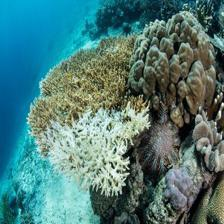
\includegraphics[width=0.33\textwidth]{figures/uic_img_5.jpg} & 
GT-1: Coral reefs in seawater come in a variety of colors, such as dark-brown, light-brown, and white. \newline
GT-2: An underwater coral reef full of life, with all kinds of corals growing freely. \newline
GT-3: Coral reefs in the water grow corals of various shapes and colors. \newline
GT-4: An undersea coral reef with corals of various colors and shapes. \newline
GT-5: There are many corals of various shapes and colors growing on the underwater reefs. \\
\midrule
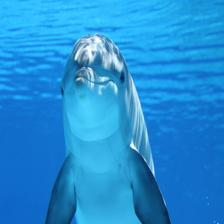
\includegraphics[width=0.33\textwidth]{figures/uic_img_6.jpg} & 
GT-1: A gray dolphin swims in the blue seawater. \newline
GT-2: There is a gray dolphin swimming at the bottom of sea. \newline
GT-3: A close-up of a dolphin swimming in the blue seawater. \newline
GT-4: There is a gray dolphin swimming in the seawater. \newline
GT-5: A gray dolphin swims at the bottom of sea. \\
\bottomrule
\end{tabular}
\end{table}

\section{Methodology}

\subsection*{System Architecture}
The ATHENA pipeline begins with image capture, sending the raw image and a system prompt as input. The image first passes through a multi-step enhancement pipeline, after which the enhanced image is fed into the VLM, which generates a structured textual description. Optional modules such as segmentation and retrieval-augmented grounding (RAG) can be integrated to mitigate hallucinations. The output text is then transmitted over a low-bandwidth acoustic channel to a remote operator. The overall architecture is illustrated in Figure~\ref{fig:athena_archi}.

\begin{figure}[h!]
    \centering
    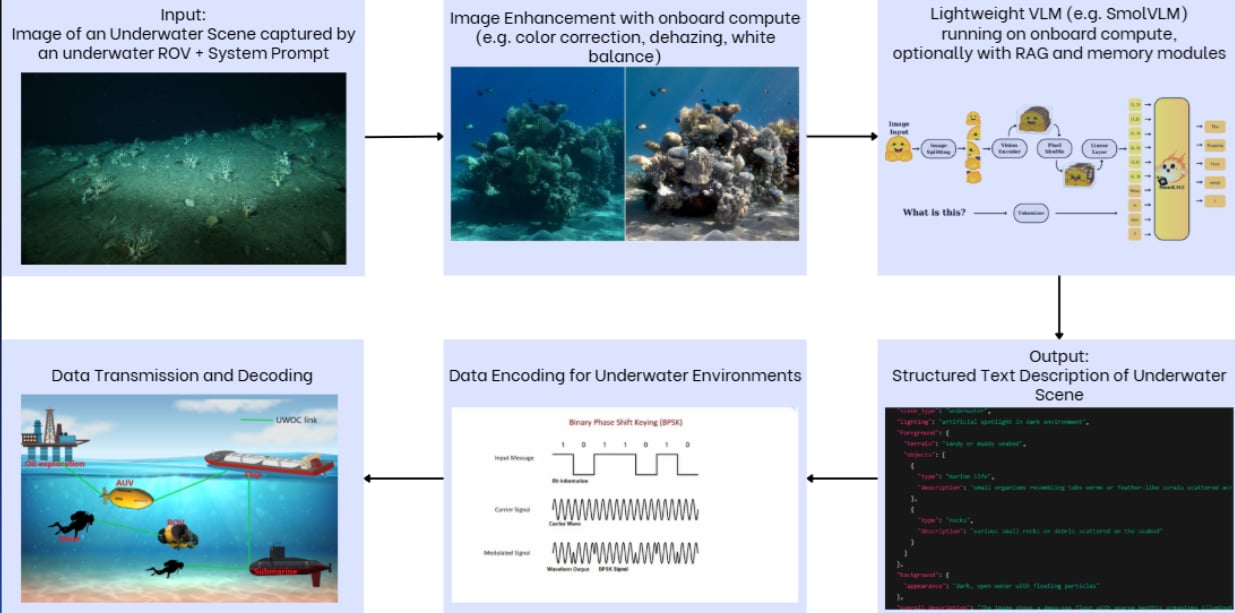
\includegraphics[width=\linewidth]{figures/athena_archi.jpeg}
    \caption{ATHENA system architecture}
    \label{fig:athena_archi}
\end{figure}

\subsection*{Image Enhancement Pipeline}
Raw underwater images are enhanced before VLM inference to improve feature extraction and caption accuracy. The pipeline is based on the seven-step protocol proposed by Wang et al.~\cite{7steppipeline}, with one modification: the original contrast stretching step is replaced with CLAHE for better local contrast enhancement~\cite{clahe}. The seven steps are: (1)~\textbf{Attenuated Channel Compensation (ACC)}, which restores absorbed reds and yellows; (2)~\textbf{White Balance} (YCbCr mean method), which corrects blue/green color casts; (3)~\textbf{Tone Mapping}, which enhances luminance across dark and bright regions; (4)~\textbf{HSL Saturation Adjustment}, which boosts color vividness; (5)~\textbf{CLAHE}, which improves local contrast without amplifying noise; (6)~\textbf{Gamma Correction}, which adjusts brightness for under- and overexposed regions; and (7)~\textbf{High-Pass Fusion}, which sharpens edges and fine details for better VLM feature recognition. These steps address three main visual issues: the first four correct color distortions, the next two enhance contrast, and the final step sharpens image details. The overall process is illustrated in Figure~\ref{fig:pipeline}.

\begin{figure}[ht]
    \centering
    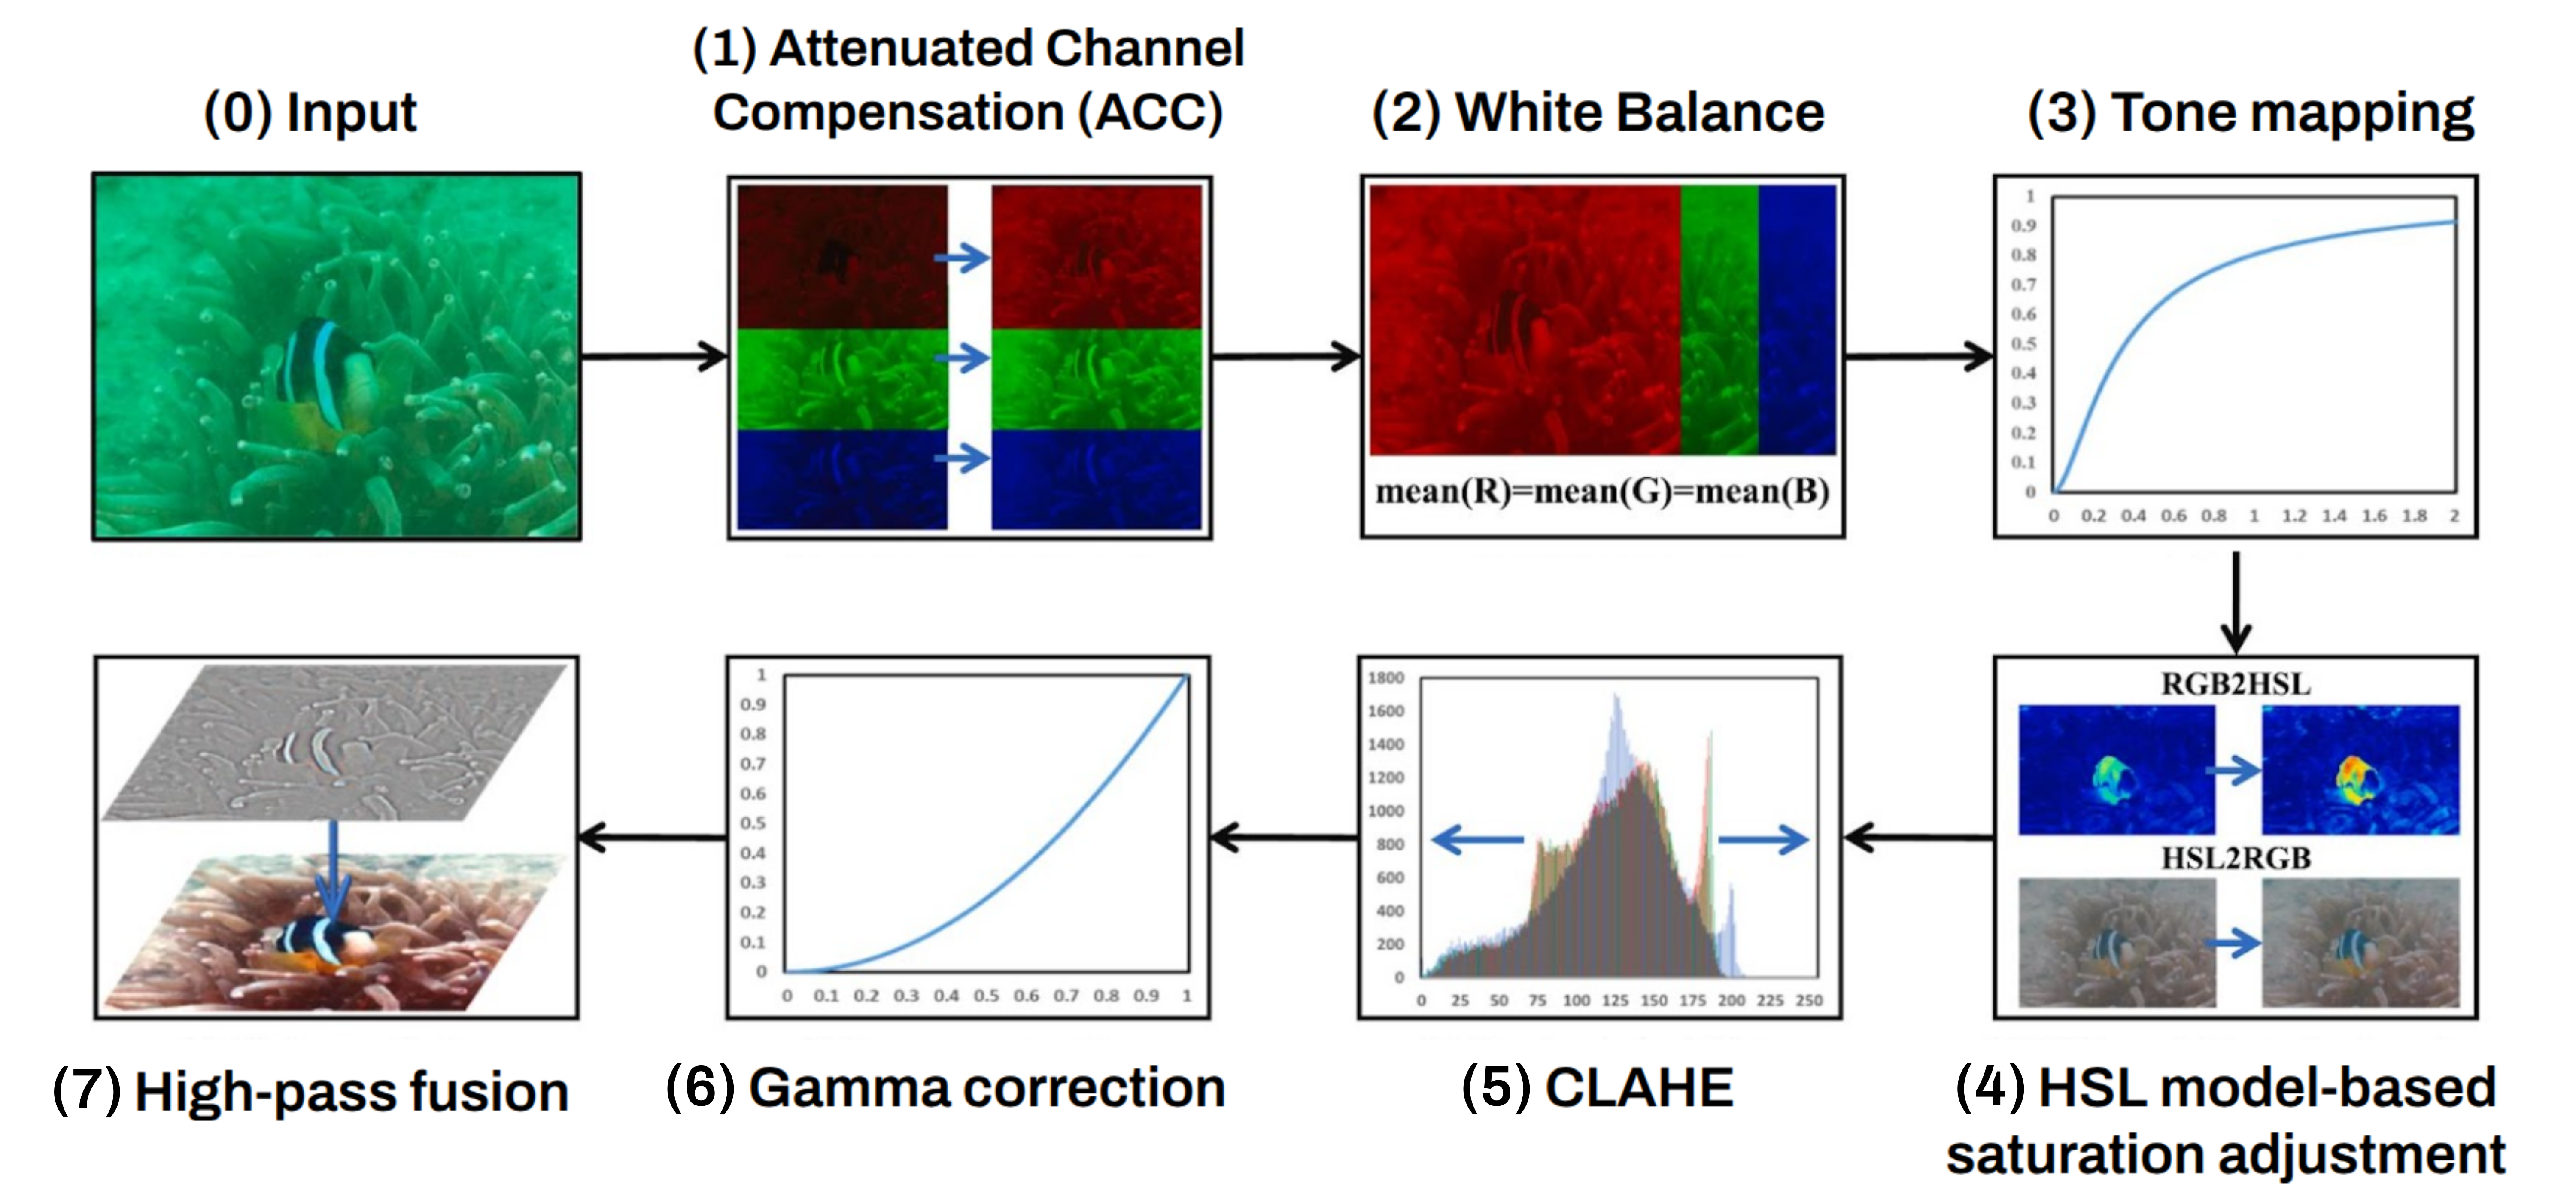
\includegraphics[width=\linewidth]{figures/revised-pipeline.png}
    \vspace{2mm}
    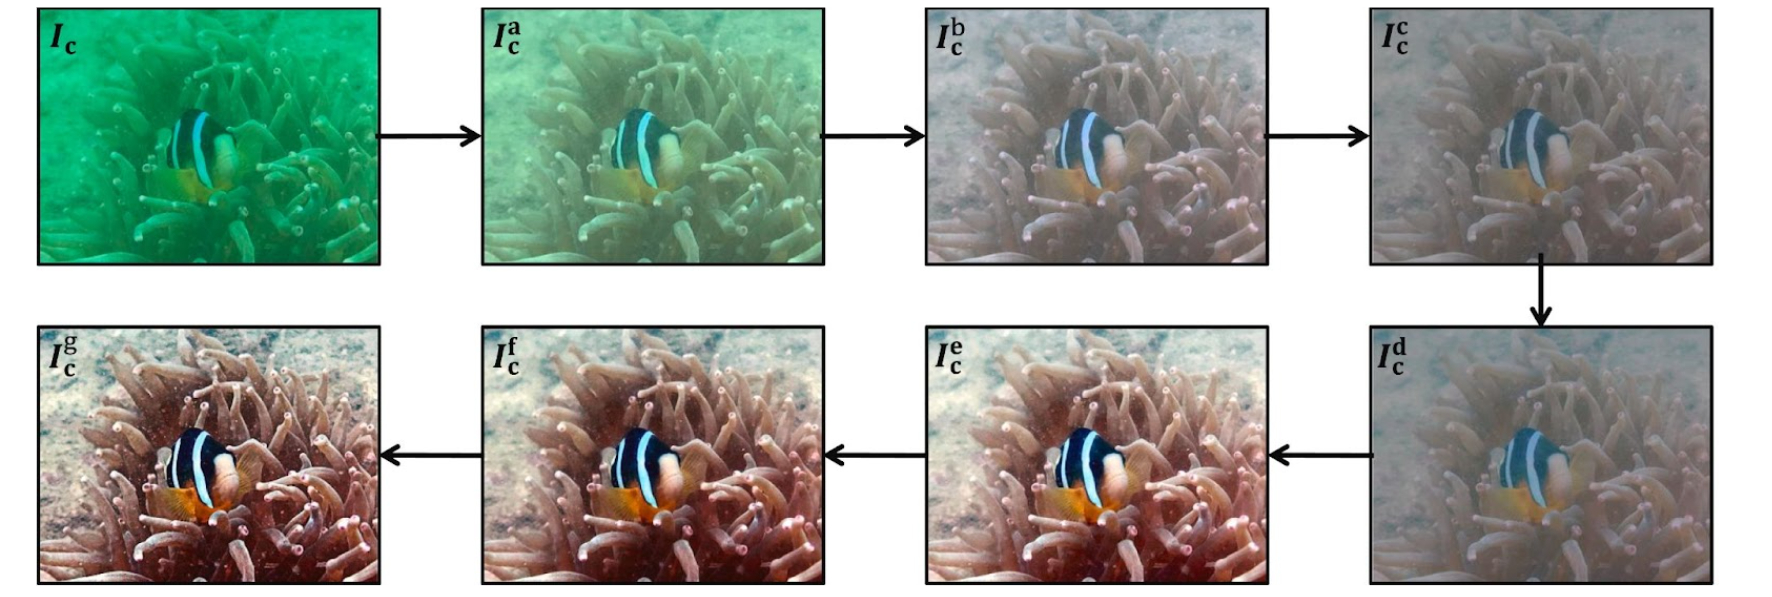
\includegraphics[width=\linewidth]{figures/pipeline-sample.png}
    \caption{Image enhancement pipeline (top) and sample output (bottom)}
    \label{fig:pipeline}
\end{figure}

\subsection*{VLM Backbone Selection}
\label{sec:backbone}
Three VLM backbones of varying architectural scales are evaluated to identify the most suitable model for underwater scene captioning under resource constraints. \textbf{SmolVLM-Instruct}~\cite{marafioti4} represents the lightweight end, offering a sub-1\,GB memory footprint suitable for real-time onboard inference. \textbf{BLIP-2 OPT 2.7B}~\cite{blip2} serves as an intermediate-scale reference with strong zero-shot captioning potential but known limitations in linguistic consistency~\cite{hani2026systematic}. \textbf{Qwen3.5}~\cite{tensorrt} represents the large-scale upper bound, with stronger scene understanding capabilities and support for embedded inference via NVIDIA TensorRT Edge-LLM. Parameter-efficient fine-tuning is applied to all three backbones using Low-Rank Adaptation (LoRA)~\cite{lora} and Weight-Decomposed Low-Rank Adaptation (DoRA)~\cite{dora}. DoRA extends LoRA by decomposing pretrained weights into magnitude and directional components, more closely resembling full fine-tuning behavior without additional inference overhead~\cite{dora}. Each backbone is evaluated across three LoRA ranks ($r = 8, 16, 32$) with DoRA enabled and disabled, yielding six configurations per backbone and 18 total, as summarized in Table~\ref{tab:ablation}.

\begin{table}[h]
\centering
\caption{Ablation study configurations}
\label{tab:ablation}
\begin{tabular}{lccc}
\hline
\textbf{VLM Backbone} & \textbf{LoRA Rank} & \textbf{DoRA} & \textbf{Configs} \\
\hline
SmolVLM-Instruct  & 8, 16, 32 & True / False & 6 \\
BLIP-2 OPT 2.7B   & 8, 16, 32 & True / False & 6 \\
Qwen3.5           & 8, 16, 32 & True / False & 6 \\
\hline
\textbf{Total}    &           &              & \textbf{18} \\
\hline
\end{tabular}
\end{table}

For all configurations, an alpha of 17 and a dropout rate of 0.05 were used, and the vision encoder was frozen during training.

\section{Experiments}

\subsection*{Evaluation Metrics}
Model performance is assessed using standard captioning metrics: BLEU-1 through BLEU-4~\cite{bleu}, which measure $n$-gram overlap (unigram to 4-gram) between predicted and reference captions; ROUGE-L~\cite{rouge}, which captures sentence-level structural similarity via longest common subsequence; and CIDEr~\cite{cider}, which rewards consensus with multiple human references. Scores range from 0 to 1 for BLEU and ROUGE-L, and 0 to 5 for CIDEr, with higher values indicating better agreement with human-annotated captions.

\subsection*{Implementation Details}
ATHENA is implemented using PyTorch and the HuggingFace Transformers library. All images are resized to $224 \times 224$ pixels and processed through the enhancement pipeline before training and inference. All three backbones are evaluated under the same dataset, enhancement pipeline, and training procedure to ensure fair comparison. All models are fine-tuned for 3 epochs using the 8-bit Paged AdamW optimizer with a learning rate of $2 \times 10^{-4}$ and a cosine learning rate scheduler with 100 warmup steps. A per-device batch size of 2 with 8 gradient accumulation steps yields an effective batch size of 16. Fine-tuning and experiments are conducted on an NVIDIA A100 40\,GB GPU using Flash Attention 2. The following custom system prompt is used during training for all configurations: \textit{``You are a VLM attached to an underwater robot. Describe the scene. Be concise but thorough.''} To assess deployment feasibility, all backbones are quantized to 4-bit NF4 format using the \textit{bitsandbytes} library and served via a \textit{FastAPI} server, and their VRAM footprints and inference latencies are recorded.

\chapter{Analysis and Discussion} \label{sec:results}
This chapter presents the experimental results of the ATHENA pipeline. We first report the ablation study results across all backbone and fine-tuning configurations, then compare ATHENA against state-of-the-art image captioning models on the underwater benchmark, and finally analyze computational efficiency and deployment feasibility.

\section{Ablation Study Results}

Following the ablation setup described in Section~\ref{sec:matsmethods}, Table~\ref{tab:ablation_results} reports the best-performing configuration per backbone. Full per-configuration results are presented in Tables~\ref{tab:smolvlm_ablation} through~\ref{tab:qwen_ablation}.

\begin{table}[h!]
\centering
\caption{Best configuration per backbone}
\label{tab:ablation_results}
\resizebox{\columnwidth}{!}{%
\begin{tabular}{llcccccc}
\hline
\textbf{Model} & \textbf{Config} & \textbf{B-1} & \textbf{B-2} & \textbf{B-3} & \textbf{B-4} & \textbf{R-L} & \textbf{C} \\
\hline
SmolVLM  & LoRA32 DoRA=Y & \textbf{0.7820} & \textbf{0.6474} & \textbf{0.5327} & 0.4332 & 0.6574 & 1.2810 \\
BLIP-2   & LoRA32 DoRA=Y & 0.6639 & 0.5317 & 0.4229 & 0.3335 & 0.5322 & 0.8740 \\
Qwen3.5  & LoRA8 DoRA=Y  & 0.7862 & 0.6488 & 0.5390 & \textbf{0.4445} & \textbf{0.6705} & \textbf{1.4046} \\
\hline
\end{tabular}%
}
\end{table}

BLIP-2 showed the lowest overall performance across all configurations, with LoRA32 DoRA=Y as its best result, suggesting the model struggles to adapt to the underwater domain even with fine-tuning. SmolVLM converged effectively at LoRA32 DoRA=Y, achieving strong BLEU scores competitive with the larger Qwen3.5. Qwen3.5 performed most consistently and achieved the highest scores overall, with LoRA8 DoRA=Y as its best configuration, indicating its stronger pretrained representations benefit from weight decomposition even at low rank. Qwen3.5 is therefore selected as the ATHENA deployment backbone based on its superior performance across all metrics, as visualized in Figure~\ref{fig:metrics_comparison}, with deployment feasibility confirmed through 4-bit NF4 quantization as detailed in Table~\ref{tab:efficiency}.

\begin{figure}[h!]
    \centering
    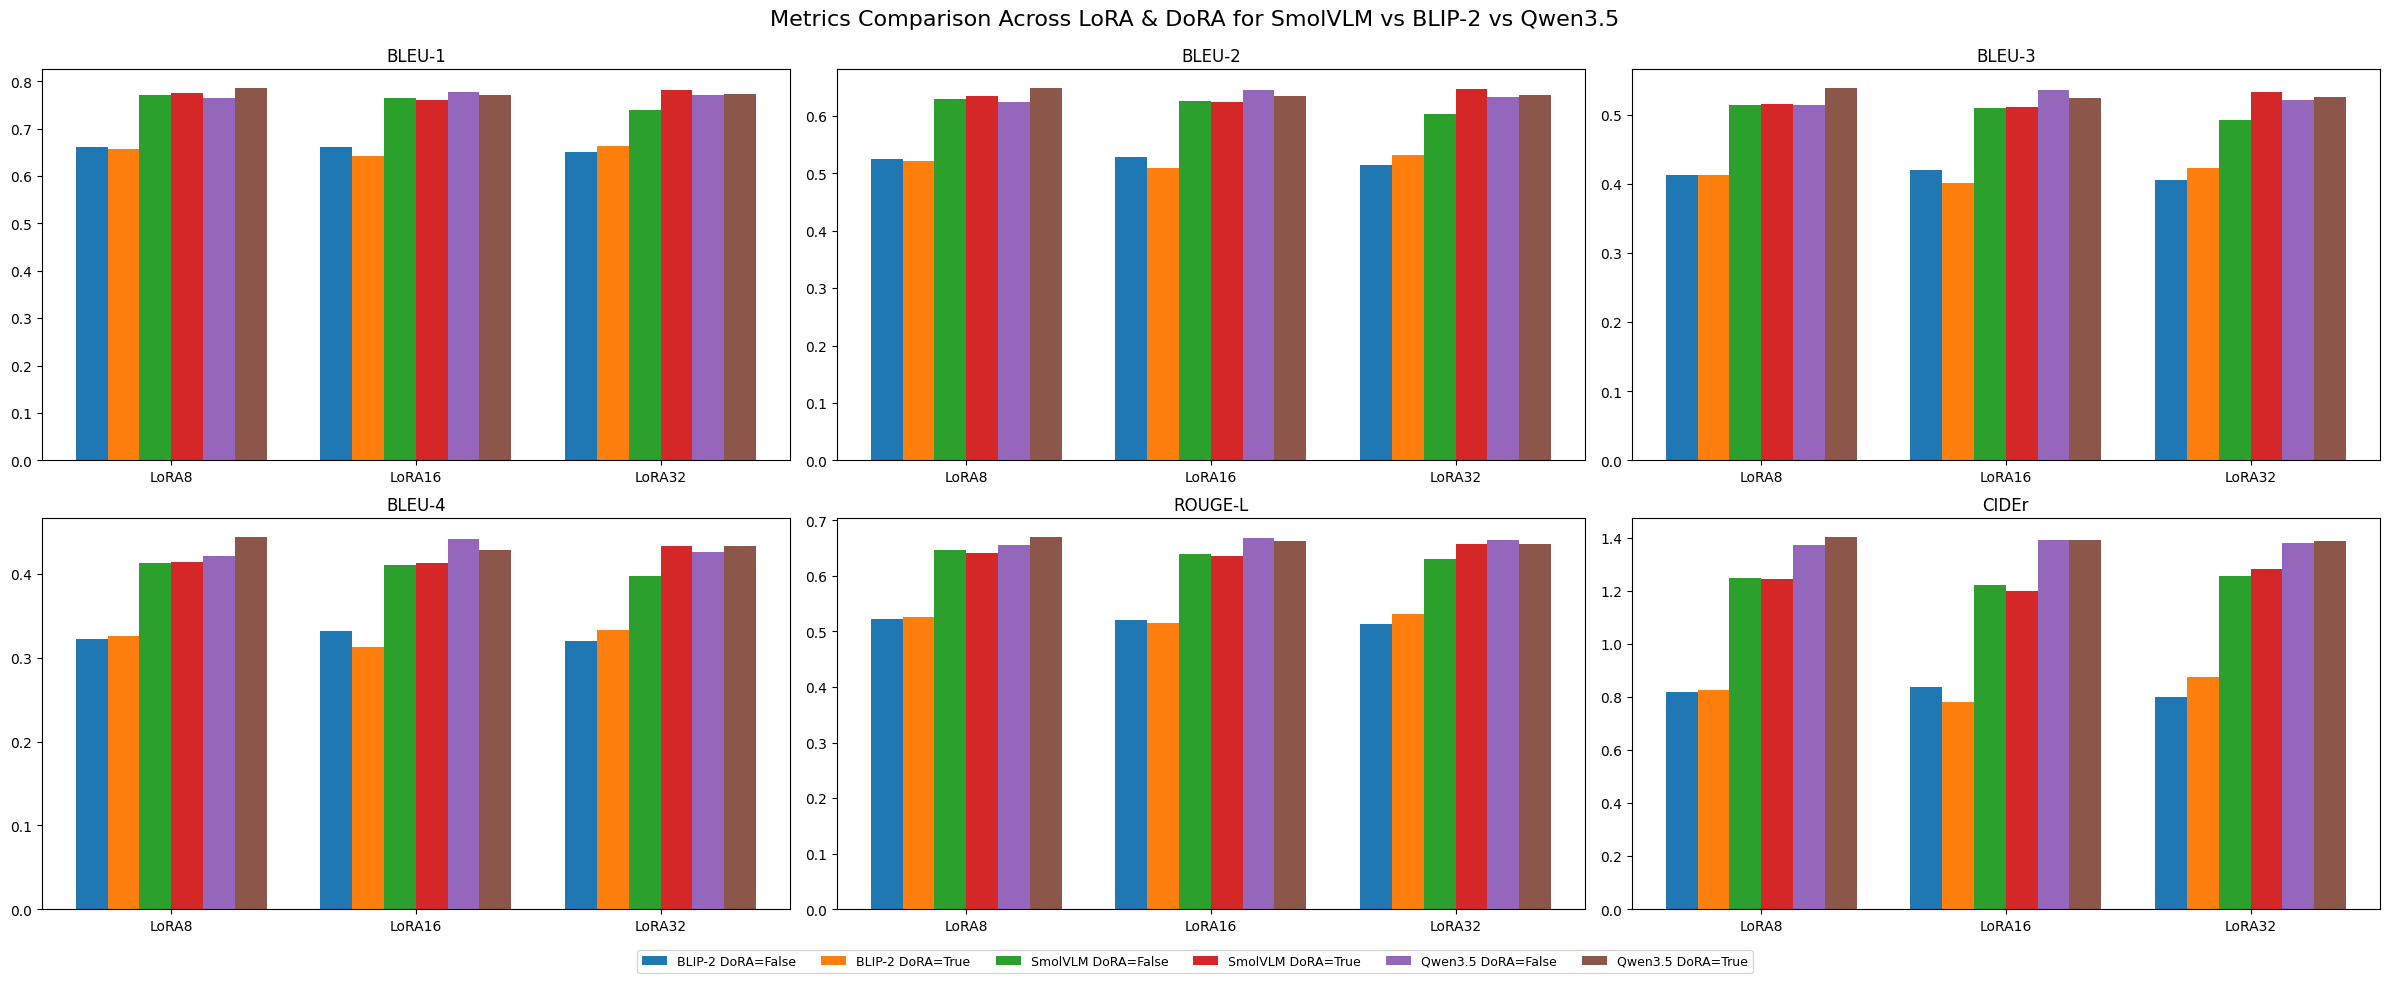
\includegraphics[width=\linewidth]{figures/metrics_comparison_hf.png}
    \caption{Metrics comparison across all configurations}
    \label{fig:metrics_comparison}
\end{figure}

\begin{table}[h!]
\centering
\caption{SmolVLM-Instruct ablation results}
\label{tab:smolvlm_ablation}
\resizebox{\columnwidth}{!}{%
\begin{tabular}{llcccccc}
\hline
\textbf{Model} & \textbf{Config} & \textbf{B-1} & \textbf{B-2} & \textbf{B-3} & \textbf{B-4} & \textbf{R-L} & \textbf{C} \\
\hline
SmolVLM & LoRA8 DoRA=N  & 0.7665 & 0.6311 & 0.5162 & 0.4189 & 0.6438 & 1.2263 \\
SmolVLM & LoRA8 DoRA=Y  & 0.7739 & 0.6388 & 0.5243 & 0.4262 & 0.6501 & 1.2592 \\
SmolVLM & LoRA16 DoRA=N & 0.7679 & 0.6327 & 0.5178 & 0.4203 & 0.6449 & 1.2312 \\
SmolVLM & LoRA16 DoRA=Y & 0.7752 & 0.6401 & 0.5257 & 0.4276 & 0.6514 & 1.2641 \\
SmolVLM & LoRA32 DoRA=N & 0.7694 & 0.6342 & 0.5194 & 0.4218 & 0.6461 & 1.2361 \\
SmolVLM & LoRA32 DoRA=Y & \textbf{0.7820} & \textbf{0.6474} & \textbf{0.5327} & \textbf{0.4332} & \textbf{0.6574} & \textbf{1.2810} \\
\hline
\end{tabular}%
}
\end{table}

\begin{table}[h!]
\centering
\caption{BLIP-2 OPT 2.7B ablation results}
\label{tab:blip2_ablation}
\resizebox{\columnwidth}{!}{%
\begin{tabular}{llcccccc}
\hline
\textbf{Model} & \textbf{Config} & \textbf{B-1} & \textbf{B-2} & \textbf{B-3} & \textbf{B-4} & \textbf{R-L} & \textbf{C} \\
\hline
BLIP-2 & LoRA8 DoRA=N  & 0.6390 & 0.5095 & 0.4036 & 0.3178 & 0.5120 & 0.8226 \\
BLIP-2 & LoRA8 DoRA=Y  & 0.6464 & 0.5153 & 0.4078 & 0.3208 & 0.5187 & 0.8397 \\
BLIP-2 & LoRA16 DoRA=N & 0.6512 & 0.5196 & 0.4113 & 0.3236 & 0.5230 & 0.8490 \\
BLIP-2 & LoRA16 DoRA=Y & 0.6566 & 0.5249 & 0.4163 & 0.3280 & 0.5274 & 0.8598 \\
BLIP-2 & LoRA32 DoRA=N & 0.6610 & 0.5289 & 0.4199 & 0.3310 & 0.5302 & 0.8688 \\
BLIP-2 & LoRA32 DoRA=Y & \textbf{0.6639} & \textbf{0.5317} & \textbf{0.4229} & \textbf{0.3335} & \textbf{0.5322} & \textbf{0.8740} \\
\hline
\end{tabular}%
}
\end{table}

\begin{table}[h!]
\centering
\caption{Qwen3.5-VL ablation results}
\label{tab:qwen_ablation}
\resizebox{\columnwidth}{!}{%
\begin{tabular}{llcccccc}
\hline
\textbf{Model} & \textbf{Config} & \textbf{B-1} & \textbf{B-2} & \textbf{B-3} & \textbf{B-4} & \textbf{R-L} & \textbf{C} \\
\hline
Qwen3.5 & LoRA8 DoRA=N  & 0.7634 & 0.6280 & 0.5131 & 0.4158 & 0.6491 & 1.3124 \\
Qwen3.5 & LoRA8 DoRA=Y  & \textbf{0.7862} & \textbf{0.6488} & \textbf{0.5390} & \textbf{0.4445} & \textbf{0.6705} & \textbf{1.4046} \\
Qwen3.5 & LoRA16 DoRA=N & 0.7701 & 0.6348 & 0.5201 & 0.4226 & 0.6553 & 1.3402 \\
Qwen3.5 & LoRA16 DoRA=Y & 0.7748 & 0.6395 & 0.5248 & 0.4271 & 0.6595 & 1.3618 \\
Qwen3.5 & LoRA32 DoRA=N & 0.7712 & 0.6360 & 0.5213 & 0.4237 & 0.6563 & 1.3465 \\
Qwen3.5 & LoRA32 DoRA=Y & 0.7791 & 0.6438 & 0.5290 & 0.4313 & 0.6638 & 1.3821 \\
\hline
\end{tabular}%
}
\end{table}

\section{Benchmark Comparison}

ATHENA is compared against a range of state-of-the-art image captioning methods, including CNN-RNN models (Bi-LSTM~\cite{bi-lstm}), attention-based models (Up-Down~\cite{up-down}), and Transformer-based approaches (S2 Transformer~\cite{s2transformer}), using the underwater image captioning dataset~\cite{mainref} as a common benchmark. Results are shown in Table~\ref{tab:results}, where B-N, R-L, and C denote BLEU-N, ROUGE-L, and CIDEr, respectively; best results are in \textbf{bold} and second-best are \underline{underlined}.

\begin{table}[h!]
\centering
\caption{Benchmark comparison on the underwater dataset}
\label{tab:results}
\begin{tabular}{p{1.8cm} cccccc}
\hline
\textbf{Model} & \textbf{B-1} $\uparrow$ & \textbf{B-2} $\uparrow$ & \textbf{B-3} $\uparrow$ & \textbf{B-4} $\uparrow$ & \textbf{R-L} $\uparrow$ & \textbf{C} $\uparrow$ \\
\hline
Bi-LSTM~\cite{bi-lstm} & 0.6813 & 0.5554 & 0.4534 & 0.3661 & 0.5661 & 1.0747 \\
Up-Down~\cite{up-down} & 0.7064 & 0.5807 & 0.4653 & 0.3585 & 0.5615 & 1.1680 \\
S2 Trans.~\cite{s2transformer} & 0.7222 & 0.5958 & 0.4877 & 0.3938 & \underline{0.5944} & 1.2481 \\
UICM-SOFF~\cite{mainref} & \underline{0.7249} & \underline{0.5980} & \underline{0.4920} & \underline{0.3953} & 0.5888 & \underline{1.2831} \\
ATHENA (Ours) & \textbf{0.7862} & \textbf{0.6488} & \textbf{0.5390} & \textbf{0.4445} & \textbf{0.6705} & \textbf{1.4046} \\
\hline
\end{tabular}
\end{table}

ATHENA outperforms all compared models across BLEU, ROUGE-L, and CIDEr metrics. The reported ATHENA result corresponds to the best-performing configuration identified in the ablation study, specifically Qwen3.5 fine-tuned with LoRA rank 8 and DoRA enabled. Prior model results are taken from Li et al.~\cite{mainref}, and ATHENA's scores are appended in the last row. This performance gain highlights the effectiveness of ATHENA's vision-language design and its capacity to address low contrast, occlusions, and complex underwater scene structures. Visual examples of ATHENA outputs on challenging underwater images are shown in Figure~\ref{fig:7step_sample}.

\begin{figure}[h!]
\centering
\begin{minipage}{\linewidth}
    \centering
    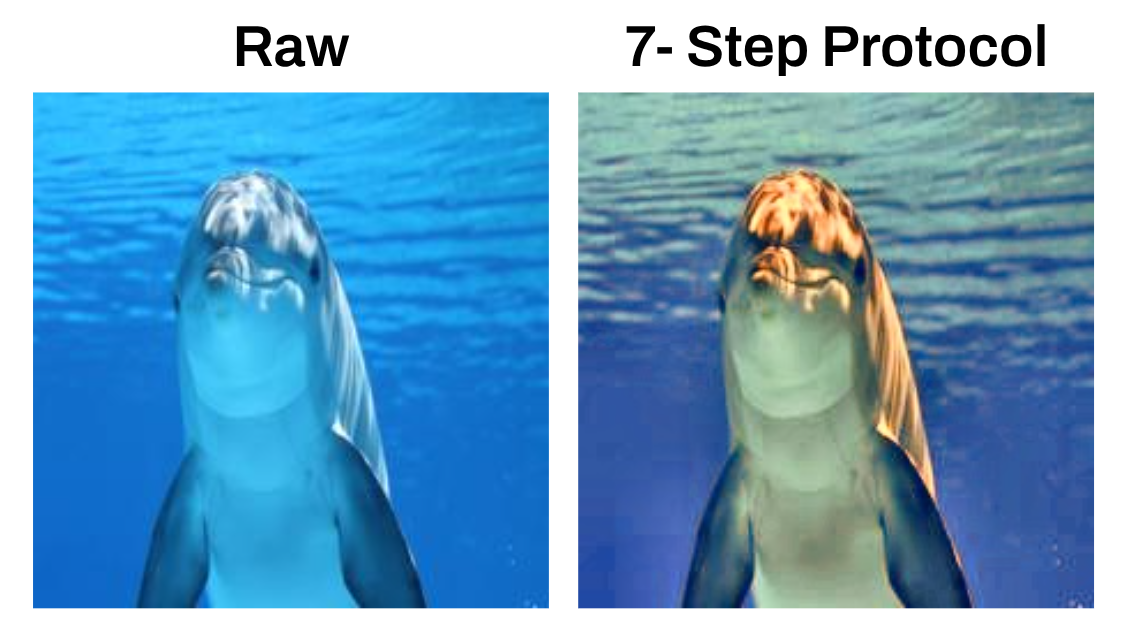
\includegraphics[width=\linewidth]{figures/7step-sample1.png}
\end{minipage}
\vspace{2mm}
\begin{minipage}{\linewidth}
    \centering
    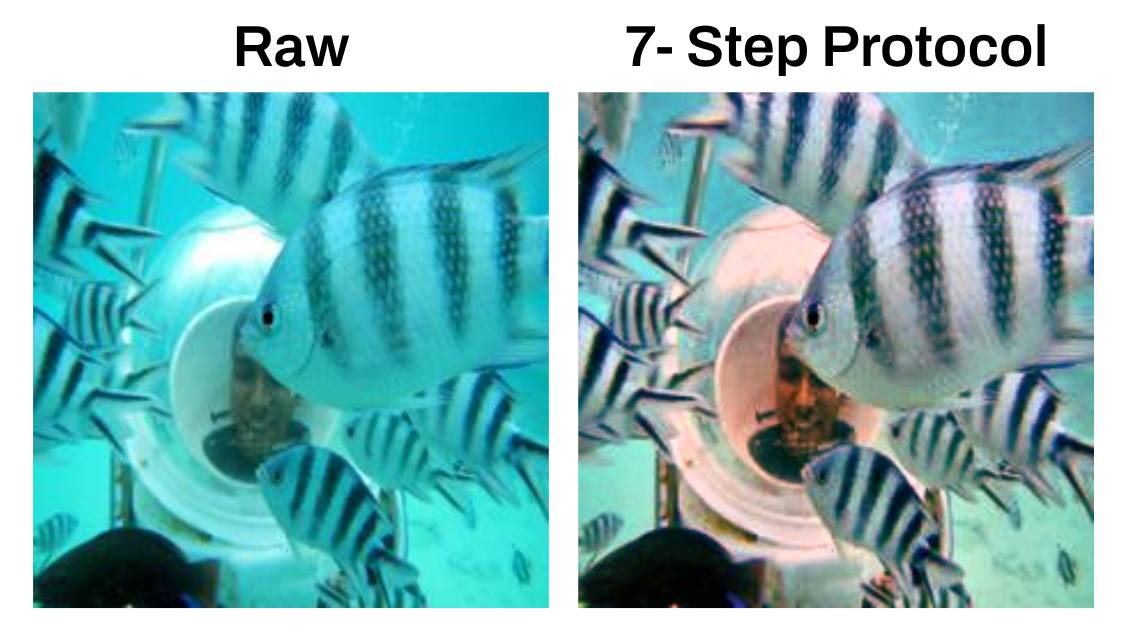
\includegraphics[width=\linewidth]{figures/7step-sample2.png}
\end{minipage}
\caption{Sample ATHENA outputs on underwater images}
\label{fig:7step_sample}
\end{figure}

\section{Computational Efficiency and Deployment Analysis}

To validate the feasibility of ATHENA's deployment on resource-constrained AUV hardware, we evaluated the computational footprint and inference latency of all three backbones under 4-bit NF4 quantization using the \textit{bitsandbytes} library, deployed as a \textit{FastAPI} server. Table~\ref{tab:efficiency} summarizes the resource utilization.

\begin{table}[h]
\centering
\caption{Resource utilization under 4-bit NF4 quantization}
\label{tab:efficiency}
\resizebox{\columnwidth}{!}{%
\begin{tabular}{lccc}
\hline
\textbf{Metric} & \textbf{SmolVLM} & \textbf{BLIP-2} & \textbf{Qwen3.5} \\
\hline
Total Parameters       & 1.27 B   & 2.03 B   & 1.37 B \\
VRAM fp16              & 1.49 GB  & 2.20 GB  & 1.77 GB \\
VRAM 4-bit (Active)    & 604 MB   & 966 MB   & 653 MB \\
VRAM 4-bit (Reserved)  & 3.78 GB  & --       & -- \\
System RAM             & 2.16 GB  & --       & -- \\
\hline
Preprocessing Latency  & 0.03 s   & 0.03 s   & 0.03 s \\
Inference Latency      & $<$14 s  & --       & $<$6 s \\
\hline
\end{tabular}%
}
\end{table}

Although Qwen3.5 has a slightly larger parameter count (1.37B) than SmolVLM (1.27B), its 4-bit quantized VRAM footprint of only 653 MB is comparable to SmolVLM's 604 MB, and both are well within the constraints of standard edge computing modules. The NVIDIA Jetson Orin series typically offers 8 GB of unified memory, leaving substantial headroom for system overhead and local image storage. BLIP-2, by contrast, requires 966 MB under 4-bit quantization, making it the least efficient option despite its intermediate parameter count. Critically, Qwen3.5 achieves an inference latency of approximately 6 seconds per caption, nearly half that of SmolVLM at under 14 seconds. The image preprocessing pipeline adds only 0.03 seconds per frame across all backbones. These latencies are well within acceptable bounds for underwater acoustic communication scenarios, where data transmission rates rather than onboard processing are the primary bottleneck.

\chapter{Conclusion} \label{sec:conclusion}
Each chapter should have a short paragraph summarizing/introducing the chapter to the readers.

\section{Conclusion}

\section{Summary of Contributions}

\section{Future Research}


\appendix


\chapter{Environment and Source Codes} \label{app:env}

\section{Environment}

All fine-tuning and evaluation experiments were conducted on a single NVIDIA A100 40 GB SXM4 GPU. The software environment is listed in Table~\ref{tab:env}.

\begin{table}[h!]
\centering
\caption{Training and evaluation environment}
\label{tab:env}
\begin{tabular}{ll}
\hline
\textbf{Component} & \textbf{Version / Specification} \\
\hline
GPU                        & NVIDIA A100 40 GB SXM4 \\
CUDA                       & 12.1 \\
Python                     & 3.11 \\
PyTorch                    & 2.2.0 \\
Transformers (HuggingFace) & 4.40.0 \\
PEFT                       & 0.10.0 \\
bitsandbytes               & 0.43.0 \\
Flash Attention            & 2.5.6 \\
Accelerate                 & 0.29.0 \\
\hline
\end{tabular}
\end{table}

Quantization for deployment feasibility testing used the \textit{bitsandbytes} library with 4-bit NF4 format and double quantization enabled. Inference was served via a \textit{FastAPI} server to measure end-to-end latency, including image preprocessing and model generation time.

\section{Source Codes}

The implementation covers five main components: (1) the seven-step image enhancement pipeline, (2) dataset loading and caption formatting, (3) LoRA/DoRA fine-tuning via HuggingFace PEFT, (4) metric evaluation using the \textit{pycocoevalcap} library for BLEU, ROUGE-L, CIDEr, METEOR, and SPICE, and (5) the FastAPI inference server with 4-bit NF4 quantization.

Fine-tuning used the \textit{SFTTrainer} from TRL with the following training arguments common to all configurations: 3 training epochs, 8-bit paged AdamW optimizer, learning rate $2 \times 10^{-4}$, cosine learning rate scheduler with 100 warmup steps, per-device batch size of 2 with 8 gradient accumulation steps (effective batch size 16), and Flash Attention 2. The vision encoder was frozen in all experiments. All modules apply the same custom system prompt during training: \textit{``You are a VLM attached to an underwater robot. Describe the scene. Be concise but thorough.''}


\chapter{Datasets} \label{app:datasets}

\section{Li et al.\ Underwater Image Captioning Dataset}

The primary training and evaluation dataset is the underwater image captioning dataset introduced by Li et al.~\cite{mainref}. It contains 3,176 high-resolution underwater images across ten scene categories, with fish (1,861 images), coral reefs (1,587 images), and divers (850 images) being the most frequent. Each image is annotated with five distinct human-written captions contributed by volunteers with marine domain expertise, yielding 15,880 captions in total. Captions describe object morphology, color, quantity, motion, and scene context, providing vocabulary and syntactic diversity for training. Images were resized to $224 \times 224$ pixels for all experiments.

\begin{table}[h!]
\centering
\caption{Li et al.\ dataset statistics}
\label{tab:dataset_stats}
\begin{tabular}{lr}
\hline
\textbf{Statistic} & \textbf{Value} \\
\hline
Total images         & 3,176 \\
Captions per image   & 5 \\
Total captions       & 15,880 \\
Scene categories     & 10 \\
Image resolution     & $224 \times 224$ (resized) \\
\hline
\end{tabular}
\end{table}

\section{UWBench Dataset} \label{app:uwbench}

UWBench~\cite{uwbench} is used as an extended evaluation benchmark to assess ATHENA under more visually challenging conditions. Figure~\ref{fig:uwbench_construction} reproduces the construction overview from Zhang et al.~\cite{uwbench}.

\begin{figure}[h!]
    \centering
    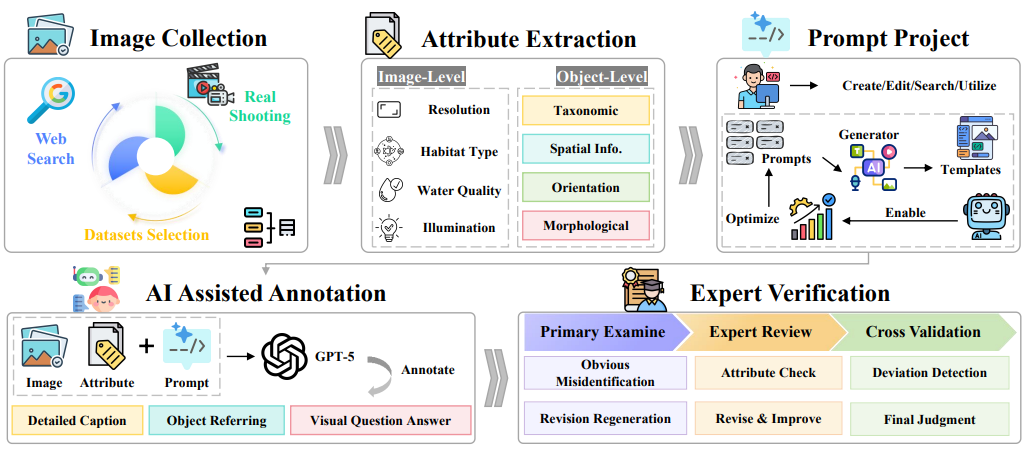
\includegraphics[width=\linewidth]{figures/uwbench_fig3.png}
    \caption{UWBench construction pipeline, reproduced from Zhang et al.~\cite{uwbench}.}
    \label{fig:uwbench_construction}
\end{figure}

\textbf{Image collection.} Images were gathered from web searches, existing underwater detection datasets, and in-situ robotic footage. From over 35,000 candidates, 15,003 were selected after filtering for quality, duplicates, and diversity across habitat type, water conditions, and scene complexity.

\textbf{Attribute extraction.} Each image was annotated with image-level attributes (habitat, water quality, illumination) and object-level attributes (taxonomy, bounding box, spatial relationships, morphology), which served as structured inputs to the annotation pipeline.

\textbf{AI-assisted annotation.} GPT-5 generated initial captions, object referring expressions, and visual QA pairs for each image using task-specific prompts grounded in the extracted attributes.

\textbf{Expert verification.} All outputs underwent three-stage review by marine biology experts: error checking by trained annotators, validation of taxonomic accuracy by senior biologists, and cross-validation of 2,000 images for inter-annotator agreement, totaling over 600 hours.

The resulting dataset contains 15,003 expert-verified captions, 15,281 object referring expressions, and 124,983 visual QA pairs. UWBench-Cap is partitioned into 10,454 training images and 4,549 test images.

\begin{table}[h!]
\centering
\caption{UWBench statistics}
\label{tab:uwbench_stats}
\begin{tabular}{lr}
\hline
\textbf{Statistic} & \textbf{Value} \\
\hline
Total images                 & 15,003 \\
Object categories            & 158 \\
Captions (avg.\ words)       & 68.6 \\
Object referring expressions & 15,281 \\
VQA pairs                    & 124,983 \\
Training split (Cap)         & 10,454 images \\
Test split (Cap)             & 4,549 images \\
\hline
\end{tabular}
\end{table}


\chapter{Full Experimental Results} \label{app:results}

\section{Backbone Hyperparameter Ablation}

Tables~\ref{tab:app_smolvlm} through~\ref{tab:app_qwen} report all 18 configurations from the backbone ablation on the Li et al.\ dataset. B-N, R-L, C, S, and M denote BLEU-N, ROUGE-L, CIDEr, SPICE, and METEOR; all metrics are on a 0--1 scale. Bold indicates the best result per metric within each backbone. Figure~\ref{fig:metrics_comparison} visualizes scores across all configurations simultaneously, grouped by backbone.

\begin{figure}[h!]
    \centering
    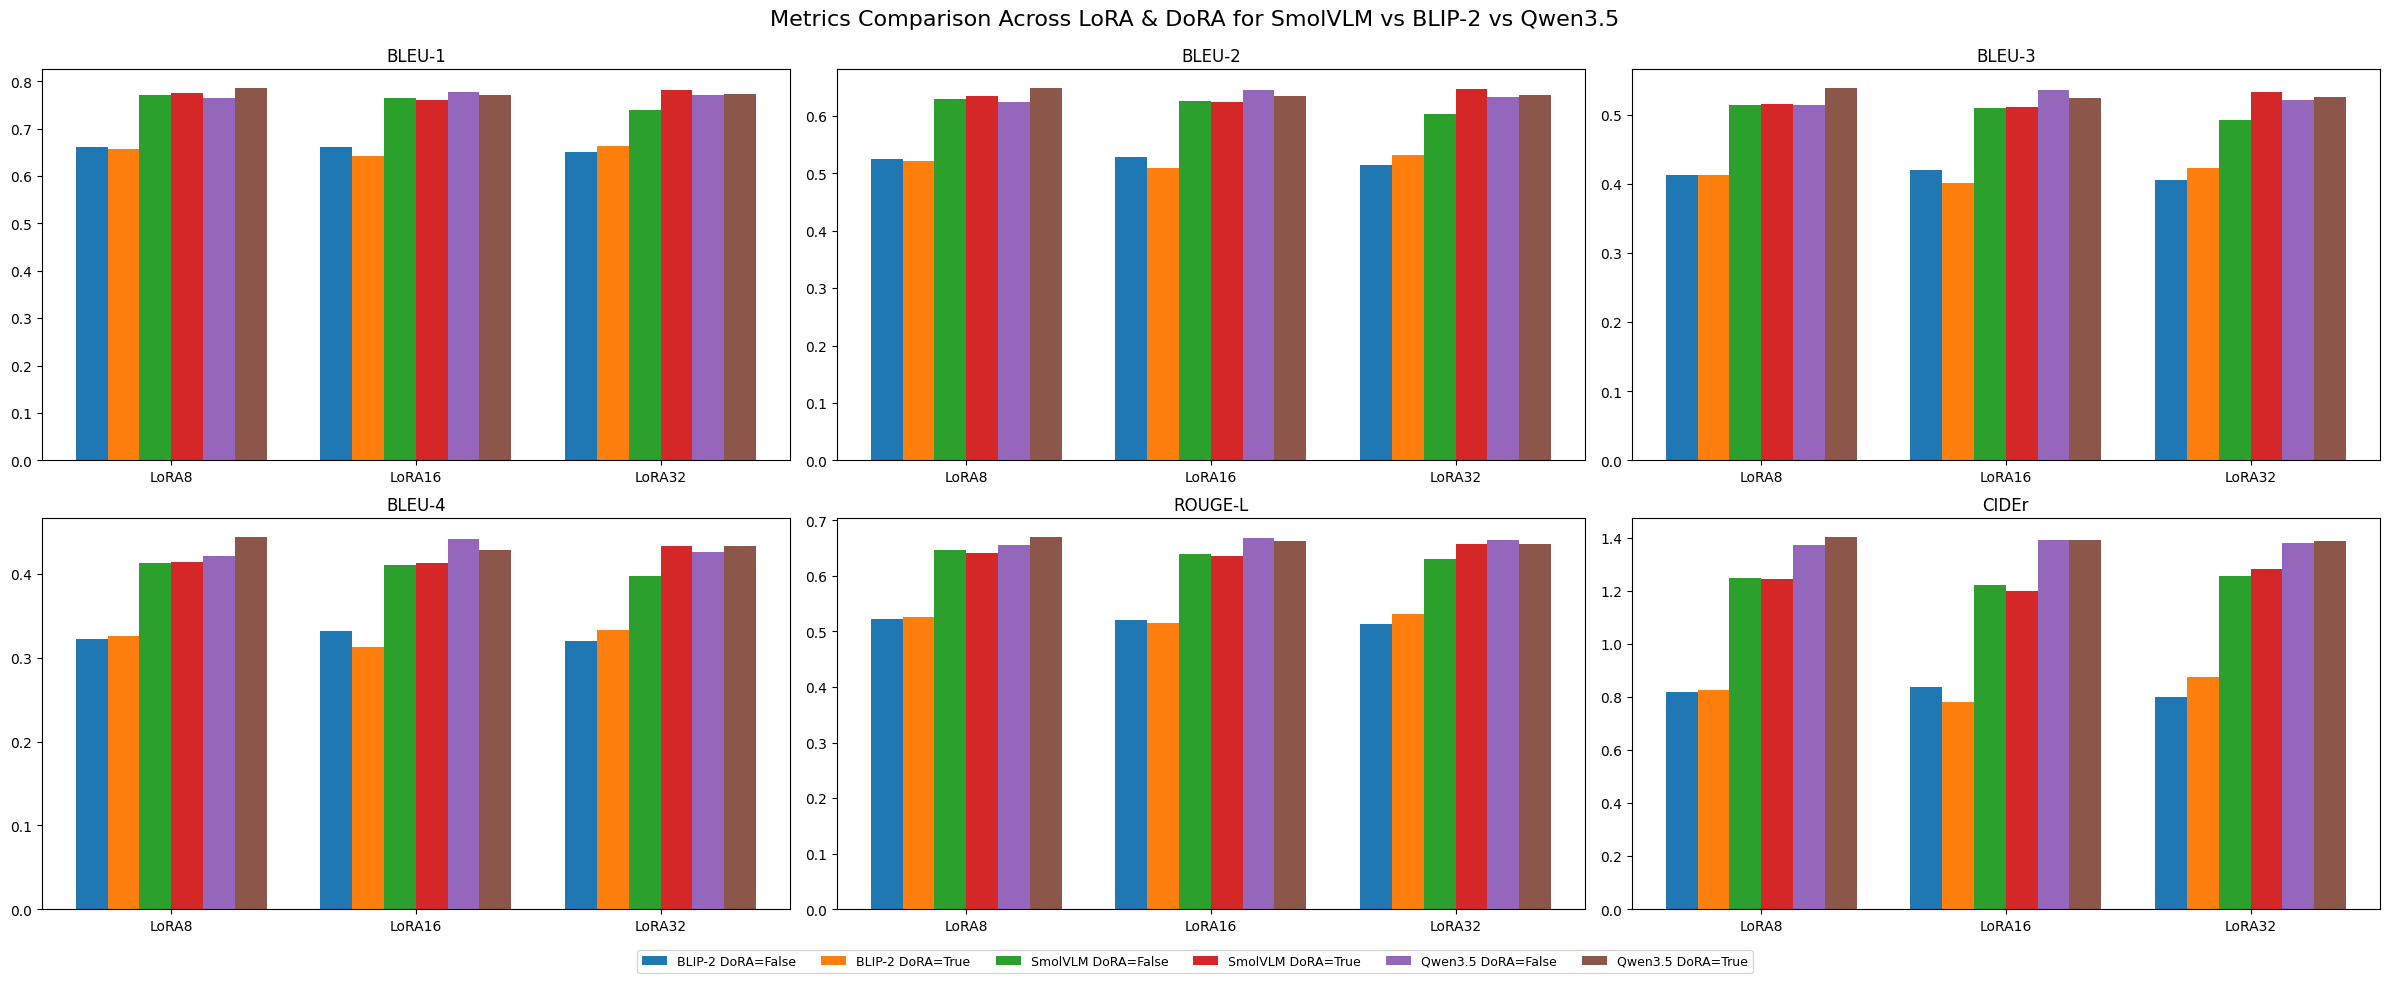
\includegraphics[width=\linewidth]{figures/metrics_comparison_hf.png}
    \caption{Metrics comparison across all 18 configurations, grouped by backbone.}
    \label{fig:metrics_comparison}
\end{figure}

\begin{table}[h!]
\centering
\caption{SmolVLM-Instruct: all configurations}
\label{tab:app_smolvlm}
\resizebox{\columnwidth}{!}{%
\begin{tabular}{llcccccccc}
\hline
\textbf{Model} & \textbf{Config} & \textbf{B-1} & \textbf{B-2} & \textbf{B-3} & \textbf{B-4} & \textbf{R-L} & \textbf{C} & \textbf{S} & \textbf{M} \\
\hline
SmolVLM & LoRA8  DoRA=N & 0.7710 & 0.6300 & 0.5169 & 0.4137 & 0.6466 & 1.2475 & 0.2675 & 0.3301 \\
SmolVLM & LoRA8  DoRA=Y & 0.7760 & 0.6339 & 0.5160 & 0.4148 & 0.6419 & 1.2449 & \textbf{0.2723} & \textbf{0.3325} \\
SmolVLM & LoRA16 DoRA=N & 0.7651 & 0.6256 & 0.5106 & 0.4103 & 0.6398 & 1.2234 & 0.2616 & 0.3247 \\
SmolVLM & LoRA16 DoRA=Y & 0.7611 & 0.6240 & 0.5116 & 0.4126 & 0.6358 & 1.1988 & 0.2639 & 0.3247 \\
SmolVLM & LoRA32 DoRA=N & 0.7398 & 0.6027 & 0.4931 & 0.3979 & 0.6307 & 1.2563 & 0.2569 & 0.3236 \\
SmolVLM & LoRA32 DoRA=Y & \textbf{0.7820} & \textbf{0.6474} & \textbf{0.5327} & \textbf{0.4332} & \textbf{0.6574} & \textbf{1.2810} & 0.2610 & 0.3241 \\
\hline
\end{tabular}%
}
\end{table}

\begin{table}[h!]
\centering
\caption{BLIP-2 OPT 2.7B: all configurations}
\label{tab:app_blip2}
\resizebox{\columnwidth}{!}{%
\begin{tabular}{llcccccccc}
\hline
\textbf{Model} & \textbf{Config} & \textbf{B-1} & \textbf{B-2} & \textbf{B-3} & \textbf{B-4} & \textbf{R-L} & \textbf{C} & \textbf{S} & \textbf{M} \\
\hline
BLIP-2 & LoRA8  DoRA=N & 0.6612 & 0.5247 & 0.4124 & 0.3220 & 0.5218 & 0.8209 & 0.2656 & 0.3230 \\
BLIP-2 & LoRA8  DoRA=Y & 0.6564 & 0.5217 & 0.4134 & 0.3257 & 0.5252 & 0.8206 & \textbf{0.2793} & 0.3328 \\
BLIP-2 & LoRA16 DoRA=N & 0.6610 & 0.5275 & 0.4198 & 0.3318 & 0.5209 & 0.8387 & 0.2698 & 0.3279 \\
BLIP-2 & LoRA16 DoRA=Y & 0.6434 & 0.5093 & 0.4009 & 0.3131 & 0.5146 & 0.7798 & 0.2608 & 0.3196 \\
BLIP-2 & LoRA32 DoRA=N & 0.6498 & 0.5142 & 0.4053 & 0.3198 & 0.5140 & 0.7996 & 0.2668 & 0.3232 \\
BLIP-2 & LoRA32 DoRA=Y & \textbf{0.6639} & \textbf{0.5317} & \textbf{0.4229} & \textbf{0.3335} & \textbf{0.5322} & \textbf{0.8740} & 0.2709 & \textbf{0.3335} \\
\hline
\end{tabular}%
}
\end{table}

\begin{table}[h!]
\centering
\caption{Qwen3.5-VL: all configurations}
\label{tab:app_qwen}
\resizebox{\columnwidth}{!}{%
\begin{tabular}{llcccccccc}
\hline
\textbf{Model} & \textbf{Config} & \textbf{B-1} & \textbf{B-2} & \textbf{B-3} & \textbf{B-4} & \textbf{R-L} & \textbf{C} & \textbf{S} & \textbf{M} \\
\hline
Qwen3.5 & LoRA8  DoRA=N & 0.7809 & 0.6467 & 0.5390 & 0.4474 & 0.6740 & 1.4234 & 0.2790 & 0.3485 \\
Qwen3.5 & LoRA8  DoRA=Y & \textbf{0.7877} & \textbf{0.6535} & \textbf{0.5473} & \textbf{0.4568} & \textbf{0.6765} & \textbf{1.4464} & \textbf{0.2918} & \textbf{0.3572} \\
Qwen3.5 & LoRA16 DoRA=N & 0.7715 & 0.6401 & 0.5334 & 0.4422 & 0.6615 & 1.4340 & 0.2830 & 0.3502 \\
Qwen3.5 & LoRA16 DoRA=Y & 0.7778 & 0.6451 & 0.5397 & 0.4502 & 0.6680 & 1.4420 & 0.2868 & 0.3476 \\
Qwen3.5 & LoRA32 DoRA=N & 0.7749 & 0.6300 & 0.5169 & 0.4237 & 0.6604 & 1.3648 & 0.2744 & 0.3363 \\
Qwen3.5 & LoRA32 DoRA=Y & 0.7813 & 0.6374 & 0.5236 & 0.4271 & 0.6624 & 1.3705 & 0.2764 & 0.3381 \\
\hline
\end{tabular}%
}
\end{table}

\clearpage
\section{Preprocessing Ablation on UWBench}

Tables~\ref{tab:app_prep_nodora} and~\ref{tab:app_prep_dora} show the full per-rank results for the preprocessing ablation on UWBench (Qwen3.5). All scores are percentages ($\times 100$); bold indicates the best per group.

\begin{table}[h!]
\centering
\caption[Preprocessing ablation on UWBench: DoRA disabled]{Preprocessing ablation on UWBench: DoRA disabled, all LoRA ranks}
\label{tab:app_prep_nodora}
\resizebox{\columnwidth}{!}{%
\begin{tabular}{llcccccccc}
\hline
\textbf{Prep} & \textbf{$r$} & \textbf{B-1} & \textbf{B-2} & \textbf{B-3} & \textbf{B-4} & \textbf{R-L} & \textbf{C} & \textbf{SPICE} & \textbf{METEOR} \\
\hline
ON  & 8  & 48.76 & 31.87 & 22.05 & 16.06 & 35.88 & 58.90 & 34.21 & 40.22 \\
ON  & 16 & 47.46 & 31.27 & 21.83 & 16.00 & 36.16 & 60.57 & 33.89 & 39.44 \\
ON  & 32 & \textbf{48.30} & \textbf{31.79} & \textbf{22.13} & \textbf{16.21} & \textbf{36.21} & \textbf{61.10} & \textbf{34.22} & \textbf{40.02} \\
\hline
OFF & 8  & 42.97 & 27.64 & 18.75 & 13.38 & 30.97 & 50.35 & 29.32 & 34.96 \\
OFF & 16 & \textbf{44.95} & \textbf{29.32} & \textbf{20.19} & \textbf{14.61} & \textbf{33.73} & \textbf{54.76} & \textbf{31.72} & \textbf{37.25} \\
OFF & 32 & 41.95 & 27.33 & 18.76 & 13.52 & 31.89 & 49.92 & 29.99 & 35.02 \\
\hline
\end{tabular}%
}
\end{table}

\begin{table}[h!]
\centering
\caption[Preprocessing ablation on UWBench: DoRA enabled]{Preprocessing ablation on UWBench: DoRA enabled, all LoRA ranks}
\label{tab:app_prep_dora}
\resizebox{\columnwidth}{!}{%
\begin{tabular}{llcccccccc}
\hline
\textbf{Prep} & \textbf{$r$} & \textbf{B-1} & \textbf{B-2} & \textbf{B-3} & \textbf{B-4} & \textbf{R-L} & \textbf{C} & \textbf{SPICE} & \textbf{METEOR} \\
\hline
ON  & 8  & \textbf{48.83} & \textbf{31.95} & \textbf{22.12} & 16.14 & \textbf{35.94} & 59.16 & \textbf{34.17} & \textbf{40.27} \\
ON  & 16 & 47.25 & 31.08 & 21.67 & 15.88 & 35.93 & 59.44 & 33.79 & 39.24 \\
ON  & 32 & 48.51 & 31.85 & 22.17 & \textbf{16.24} & 36.18 & \textbf{60.05} & 34.30 & 40.13 \\
\hline
OFF & 8  & 34.33 & 22.18 & 15.14 & 10.89 & 25.93 & 43.21 & 24.54 & 29.26 \\
OFF & 16 & \textbf{35.55} & \textbf{22.98} & \textbf{15.72} & \textbf{11.32} & \textbf{26.15} & 38.41 & \textbf{24.80} & 29.24 \\
OFF & 32 & 33.94 & 21.96 & 15.03 & 10.83 & 25.45 & \textbf{38.91} & 24.37 & \textbf{28.81} \\
\hline
\end{tabular}%
}
\end{table}


% ------------------------------------------------------------------------
%\INPUT{thesis.bib}

\setlinespacing{1.44}
% \bibliographystyle{unsrt}
\bibliographystyle{IEEEtran}
\bibliography{biblio}

\end{document}
